\chapter{Hormone Communications}
\label{hormones}

\nocite{Salemi2001}

\section{Biological hormones}
\label{bio_hormones}

A hormone is a biochemical that a multicellular organism generates for regulation and communication between its different organs and tissues \cite{hormones_wikipedia}.\\

Hormones are generated by glands inside the living being body, and transported by the circulatory system to the receptors on the distinct organs and tissues. Some of them are soluble in water, and are delivered to their destination through the bloodstream, meanwhile other need to be bonded to carrier proteins in order to reach the receptors.\\

The use of hormones is the main method of communication between organs and tissues in multicellular organisms, and their function is to regulate distinct physiological functions, such as digestion, respiration, growth, circadian rythms (related to sleep), mood swings, inmune system control, hunger, sexual arousal, etc.\\

Organs and tissues have proteins that act as receptors for hormones, and when a hormone is bond to them they produce a signal that leads to the activation of certain genes that regulate protein synthesis. This synthesis may produce other hormones that trigger different reactions in other organs or tissues, such as the gland that generated the first hormone, working as a homeostatic negative feedback mechanism for controlling hormone generation. The hormone concentration required to produce a reaction on the receptor is very small, and big amounts of hormones in the organism usually leads to disorders, such as under/overgrowth.\\

An interesting feature of hormone communication is that a single type of hormone can trigger different reactions depending on the organ or tissue that receives them. For example, insulin, a hormone produced by the pancreas controls the intake of glucose from blood in liver and muscle, and the intake of lipids and synthesis of triglycerides in adipocytes, as well as other anabolic effects. \\

\section{Concept of digital hormone}
\label{hormone_concept}

Digital hormones are a nature-inspired communication method first used by Wei-Min Shen, Behnam Salemi and Peter Will, researchers from the University of Southern California in 2000 \cite{Shen2000a}. They define a digital hormone as \emph{``a signal, based on biological hormones, that is able to trigger different actions at different receivers, delegating the execution of those actions to the receiver subsystems''}. In this aspect they behave just as biological hormones, like insulin, that can produce different reactions, like the intake of glucose or lipids depending on the organ that receives them. \\

A control based on digital hormones is a control that lies between a master and a masterless control. The robot can be controlled entirely by the flow of hormones, in a masterless way, or with the help of the hormones, with any module assuming the role of master module whenever is required by the robot, depending on what method is more eficient at that certain moment.\\

The main properties of digital hormones, as described by Shen, Salemi and Will are the following ones:

\begin{enumerate}
	\item {\bfseries Hormones do not have a fixed destination, but float in a distributed system}.
	
	 Since the modules do not posess a unique ID or address to identify them, hormones can not be sent to a particular module as it could be done with a standard communication protocol, such as TCP/IP. They are instead released in the system and relayed, modified or destroyed by the different nodes that receive the hormones.
	
	Even though hormones can not be sent to a concrete module, they can be sent to a module with a certain role, for example, a head module, a limb module or a spine module, and reach them by travelling through the distributed system, without any need for an ID or address, and even without knowing beforehand the route that the hormone must traverse to reach those modules.\\
	
	\item {\bfseries Hormones have a lifetime.}
	
	 In order to prevent the hormones from circulating indefinitely along the distributed system, they have a limited lifetime.
	
	A hormone can be terminated in three possible ways: when they reach their destination, when their lifetime expires, or when they reach a module with no outlinks and, therefore, they can not be relayed again to any other module.
	
	If the modular robot were to have a configuration with loops, a hormone without lifetime could be trapped in those loops indefinitely, or returned to the module that generated it, producing undesired or unexpected effects to the robot.\\
	
	\item {\bfseries The same hormone can trigger different actions in different receiving sites. }
	
	Like their biological counterparts, digital hormones can trigger diffrent actions depending on the receptor they arrive to. These actions can be either hormone modification and relay, execution of local actions, or destruction of the hormone.
	
	For example, a hormone with a limb module as destination, generated at the spine module, can trigger a relay action if it arrives to a spine module, and later trigger a movement of the module joint when the same hormone arrives to a limb module.

\end{enumerate}
~\\

In the original work of Shen, Salemi and Will, they define three kinds of hormones, that perform three different tasks: action specification, synchronization and dynamic grouping.\\

As mentioned in chapter \ref{config_gait}, the locomotion of modular robots is almost always controlled by gait tables, containing the joint values for each DOF of each module in the robot at each step of the gait. Depending on the configuration and the number of modules, this table can become very large, and sometimes redundant. By using hormones for action specification, these gait tables can be simplified to a great extent. For example, for achieving linear locomotion in a caterpillar configuration, the module next to the first one sets the same value for its joints as the last value the first module had at the previous step, and so on. Instead of storing a gait table for all the different modules, we can just store the values for the joints of the first module, and then propagate them along the caterpillar using hormones. This method also allows to add new modules to the configuration dynamically, with no need of modifying the gait table to add any new entry.\\

Synchronization is a inherent problem of a distributed system, in which many machines coexist with their own clocks and local times that have to colaborate. This problem is more evident in modular robotics, as the different modules need to be synchronized in order to generate a suitable gait for its locomotion.\\

In a distributed system with a master node, synchronization usually involves a high communication cost, since a part of the limited bandwidth is consumed in synchronization messages. On the other hand, masterless control often makes the unrealistic assumption that all modules' internal clocks are synchronized. As hormones can wait at a module until the occurrence of a certain event, such as that all local actions are finished, they can be employed as synchronization tokens.\\

For instance, in order to synchronize the steps of a caterpillar configuration, a synchronization hormone can be defined, that is sent to the next module when all the local actions have been performed. This method ensures that all modules have completed the tasks of each step before relaying the hormone to the next module. When the last module receives this hormone and finishes its job, it can send back a hormone that can be used by the head module to generate another synchronization hormone, starting again the process.\\


\section{Hormones in Hormodular}
\label{hormone_hormodular}

Modular robots in this thesis achieve locomotion through a set of sinusoidal oscillators with a certain amplitude ($A_i$), offset ($O_i$) and phase ($\phi_i$), and a global oscillation period ($T_{osc}$) shared by all the modules. The optimal values for those oscillator parameters are obtained using evolutionary optimization algorithms, maximizing the point-to-point distance travelled by the robot during a certain evaluation time, that is, the average speed of the locomotion gait.\\

Those values are later set in gait tables, one per configuration. Therefore, each module needs to know what is its current function, based on their location inside the configuration,  as well as their global configuration in order to select the appropriate parameters in the gait table corresponding to that configuration.\\

For that purpose the modules will be using digital hormones as their communication method because of the characteristics mentioned in the previous sections. This will also allow us to implement a homogeneous controller, identical for all the modules, reducing the complexity of the system, and making it much easier to maintain, control and debug.\\ 

The algorithm for module function and configuration discovery is based on three different types of hormone: a ``Ping'' hormone, in charge of the local configuration discovery and ``Leg'' and ``Head'' hormones, whose function is the global configuration discovery and communication. The next sections will describe these hormones used in the robot, as well as the communication protocol based on digital hormones, used to calculate the IDs required to select the correct gait table and oscillator parameters $A_i$, $O_i$, $\phi_i$ and $T_{osc}$ from that gait tables.
%and how to calculate the IDs required to select the correct gait table and oscillator parameters $A_i$, $O_i$, $\phi_i$ and $T_{osc}$ from that gait tables.

\subsection{Structure of a hormone}
\label{hormone_structure}

The structure of the hormones used in this thesis is the following:
\Cpp
\begin{lstlisting}
 class Hormone 
 {
 	int type; //-- Posible values: PING_HORMONE, LEG_HORMONE, HEAD_HORMONE
 	int sourceConnector; //-- Possible values: 0, 1, 2, 3
 	string data;
 };
\end{lstlisting}
\noindent \textit{  (This is a simplified implementation to show the hormone general structure. More details about the actual implementation on the Hormone.hpp file of project Hormodular.)}\\

The variable \textbf{type} defines the type of hormone, that can be either a ``Ping'' hormone, a ``Leg'' hormone or a ``Head'' hormone. These three types are explained in section \ref{hormone_types}.\\

The variable \textbf{sourceConnector} stores information about the connector that sent the hormone. This information is encoded as follows: Front connector: 0, Right connector: 1, Back connector: 2, Left connector: 3.\\

The variable \textbf{data} stores all the remaining information that might be needed, stored as a string:
\begin{itemize}
	\item ``Ping'' hormones store in \textbf{data} the local orientation of the sender module. For a sender module with roll=90º, pitch=180º and yaw=270º, \textbf{data} would contain the string: ``90 180 270''.
	
	\item ``Leg'' hormones do not need to store any extra information on \textbf{data}.
	
	\item ``Head'' hormones store two values: the first one is the ID of the configuration ( e.g. 1 for ``Tripod'' configuration) and the second one is a integer value used to discriminate the ID of each of the ``Leg'' modules.
\end{itemize}
~\\

\subsection{Types of hormones}
\label{hormone_types}
The three types of hormones used in this work differ from those three types defined by Shen, Salemi and Will in their publications, as they are used for discovering the function of each module in the locomotion gait, based on the general configuration and on the position inside that configuration to later select the oscillation parameters. These hormones are named ``Ping'' hormones, ``Leg'' hormones and ``Head'' hormones, and will be described in this section.\\

\subsubsection{``Ping'' hormones}
\label{hormone_types_ping}

``Ping'' hormones are used by the modules to discover their orientation with respect to the neighbor modules, as well as how are they connected between them. They are also used to know which connectors are active, that being the reason we have named them ``Ping'' hormones.\\

These hormones are generated by all modules and have a very short range, they only travel to the nearest neighbors of the module. Apart from the information about the connector that sent them, they include the initial orientation of the sender module in their \textbf{data} field.\\

Section \ref{hormone_algorithm_ping} explains in detail how the ``Ping'' hormones are used to calculate the local ID of the module.\\ 


\subsubsection{``Leg'' hormones}
\label{hormone_types_leg}

``Leg'' hormones are generated at the ``leg'' modules, and are used to recognize the global configuration of the modular robot. ``Leg'' modules are those who are connected to just one module, and in all the three configuration correspond to the modules in the extreme of the limbs.\\

``Leg'' hormones travel through the robot body until they arrive to the ``head'' module, which then discovers the current configuration from the amount of ``Leg'' hormone received. This process is explained in detail in section \ref{hormone_algorithm_leg}.\\


\subsubsection{``Head'' hormones}
\label{hormone_types_head}

``Head'' hormones are generated by the ``head'' modules, the module which receives ``head'' hormones at all its active connectors.\\

They flow in the opposite direction than the ``leg'' hormones, from ``head'' to ``leg'' modules and accomplish a dual function: they communicate to the rest of the modules the current global configuration discovered by the ``head'' module, and help the ``leg'' modules to distiguish among them, something that cannot be done only with the neighbors info (for the considered configurations).\\

The complete explanation of how these hormones are used can be found on section \ref{hormone_algorithm_head}.\\

\subsection{Hormone communication algorithm}
\label{hormone_algorithm}

This section explains the hormone conmmunication algorithm used by the modules to know which values they have to select from the gait table in order to achieve the optimal locomotion gait previously obtained through evolutionary algorithms. This algorithm has three main parts, one per type of hormone: local topology discovery, global configuration discovery and global configuration communication and leg discrimination.\\

\subsubsection{Local topology discovery}
\label{hormone_algorithm_ping}
For local topology discovery, i.e., discovering how a module is connected to its neighbor modules, the modules use ``Ping'' hormones. The procedure is as follows:\\

Each module sends ``Ping'' hormones through all its connectors. These hormones have information about the connector used to send them, as well as the local orientation of the sender module, obtained from the Inertial Measurement Unit (IMU) at the robot startup.\\

Only the connectors that have other modules attached to them (i.e. active connectors) will succeed in sending and receiving the hormones.\\

Each $T_{com}$ seconds, the module looks for ``Ping'' hormones at each of its connector input buffers, and calculates the module ID of each module as described in section \ref{config_repy_description}.\\

Let us consider, for instance, two modules with the configuration of figure \ref{fig:hormone_protocol_01}, in which the front connector of module 0 is connected to the back connector of module 1, and vice versa. \\

\begin{figure}[h]
	\centering
	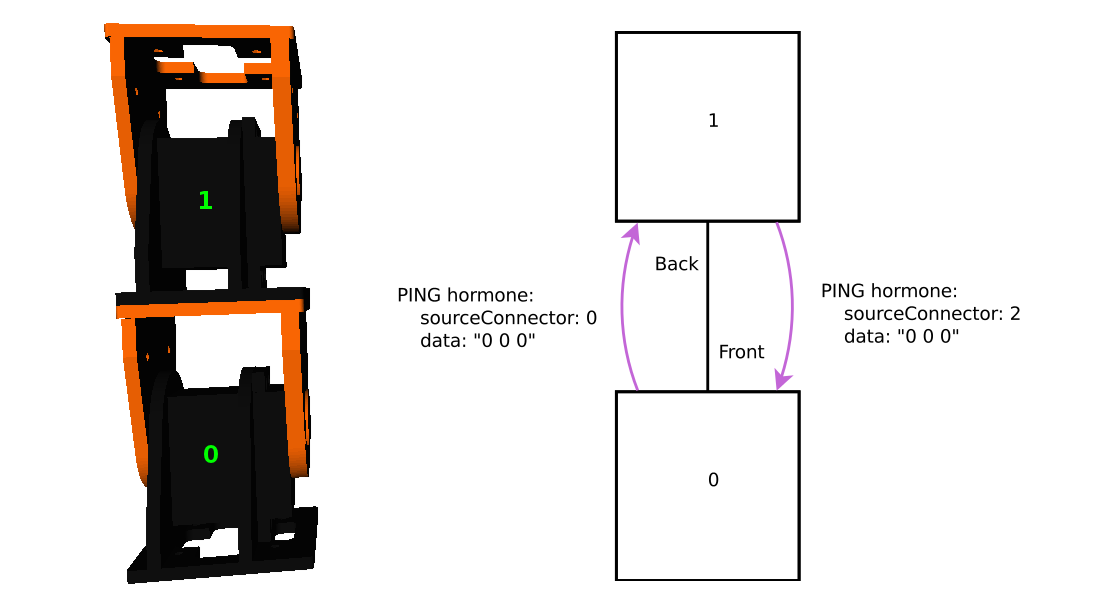
\includegraphics[width=0.7\textwidth]{images/Hormone_protocol_01.png}
	\caption{Local topology discovery in a two module configuration}\label{fig:hormone_protocol_01}
\end{figure}

For the discovery of the local topology, the module 0 would send hormones from all its connectors but, as only the front connector is attached to other module, only the hormones on the output buffer of the front connector would be delivered to module 1. The same is true for module 1, only the hormones in the back connector are able to arrive to other modules.\\

As the orientation of both modules is the same ( roll=0º, pitch=0º and yaw=0º), the \textbf{data} field in the hormones generated by both modules would be also the same: "0 0 0". \\

Each $T_{com}$ seconds, module 0 will look for ``Ping'' hormones at its input connector buffers, finding only the hormone sent by module 1. Using the information about which connector did receive the hormone (the front connector, encoded as `0'), which connector sent the hormone (the back connector, encoded as `2') and which was the remote orientation, (0º, 0º, 0º),  the module can then identify its local topology, and calculate its ID:

\[ ID = ( x_0^0 \cdot 4^0+ x_1^0 \cdot 4^1) \cdot 17^0 +
 ( x_0^1 \cdot 4^0+ x_1^1 \cdot 4^1) \cdot 17^1 +
  ( x_0^2 \cdot 4^0+ x_1^2 \cdot 4^1) \cdot 17^2 +
   ( x_0^3 \cdot 4^0+ x_1^3 \cdot 4^1) \cdot 17^3 \]
\[ ID = ( 2 \cdot 4^0 + 0 \cdot 4^1 ) \cdot 17^0 +
 16 \cdot 17^1 +
 16 \cdot 17^2 +
 16 \cdot 17^3 = 83506 \]\\
 
 Module 1 will find only the hormone from module 0, with the receptor connector info (back connector, `2'), the sender connector info (front connector, `0') and the orientation of the module, (0º, 0º, 0º). The corresponding ID for this module will be:

\[ ID = ( x_0^0 \cdot 4^0+ x_1^0 \cdot 4^1) \cdot 17^0 +
 ( x_0^1 \cdot 4^0+ x_1^1 \cdot 4^1) \cdot 17^1 +
  ( x_0^2 \cdot 4^0+ x_1^2 \cdot 4^1) \cdot 17^2 +
   ( x_0^3 \cdot 4^0+ x_1^3 \cdot 4^1) \cdot 17^3 \]
\[ ID = 16 \cdot 17^0 +
 16 \cdot 17^1 +
 ( 0 \cdot 4^0 + 0 \cdot 4^1 ) \cdot 17^2 +
 16 \cdot 17^3 = 78896 \]\\
 
The same algorithm applies to modules with more than one module connected, such as the configuration on figure \ref{fig:hormone_protocol_02}. In this case, the module 0 will receive three hormones from the neighbor modules: a hormone sent by module 1 from the back connector (`2') and received at the back connector (`2'), with a orientation of (0º, 90º, 0º), another sent by the module 2 from the back connector (`2'), received at the left connector (`3'), with a orientation of (270º, 0º, 90º) and a third one sent by the module 3 from its back connector (`2'), received at the right connector (`1'), with a orientation of (90º, 0º, 270º).\\
 
\begin{figure}[h]
	\centering
	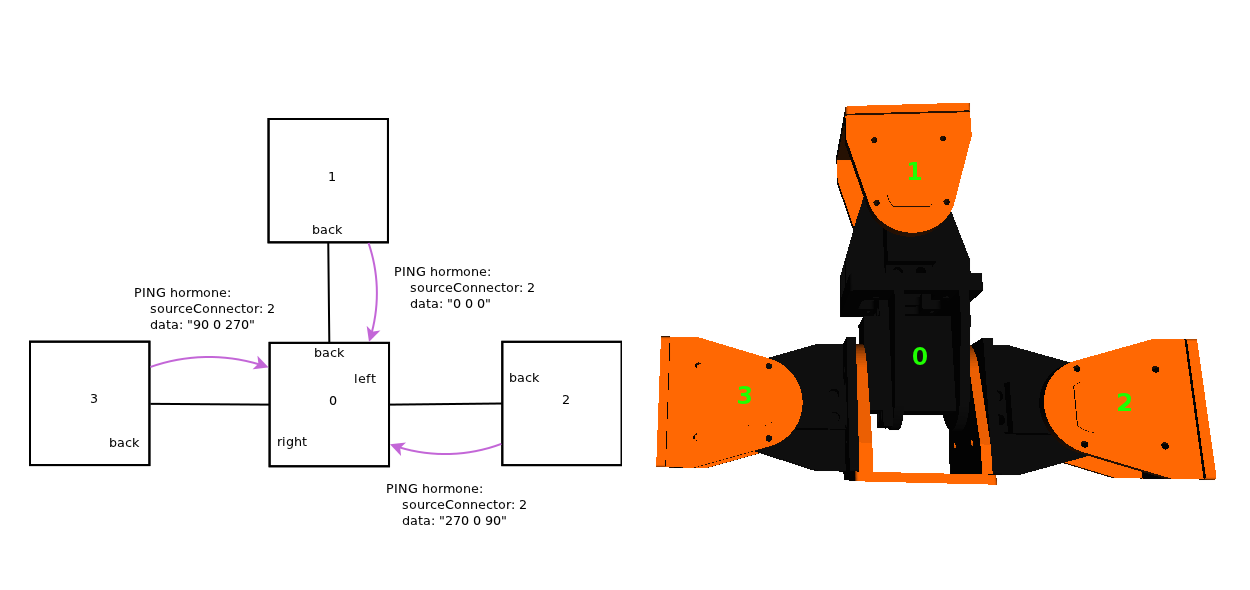
\includegraphics[width=1\textwidth]{images/Hormone_protocol_02.png}
	\caption{Local topology discovery in a four module configuration}\label{fig:hormone_protocol_02}
\end{figure}

With all this data the module 0 can calculate its ID:
\[ ID = ( x_0^0 \cdot 4^0+ x_1^0 \cdot 4^1) \cdot 17^0 +
 ( x_0^1 \cdot 4^0+ x_1^1 \cdot 4^1) \cdot 17^1 +
  ( x_0^2 \cdot 4^0+ x_1^2 \cdot 4^1) \cdot 17^2 +
   ( x_0^3 \cdot 4^0+ x_1^3 \cdot 4^1) \cdot 17^3 \]
\[ ID = 
 16 \cdot 17^0 +
 ( 2 \cdot 4^0 + 3 \cdot 4^1 ) \cdot 17^1 +
 ( 2 \cdot 4^0 + 1 \cdot 4^1 ) \cdot 17^2 +
 ( 2 \cdot 4^0 + 1 \cdot 4^1 ) \cdot 17^3 = 31466 \]\\
 
This calculated ID is unique for all modules in the three different configurations considered, except for the ``leg'' modules, which all share the same ID. For this reason we need more data in order to discriminate among the different ``leg'' modules and know their exact position inside the robot.\\
 
\subsubsection{Global configuration discovery}
\label{hormone_algorithm_leg}
``Leg'' hormones are in charge of the global configuration discovery, i.e. recognize which is the general arrangement of the modules: a tripod configuration, a quadruped configuration, etc.\\

These hormones are generated at the ``leg'' modules (those who have only one active connection with other module) and they travel along the robot by the child connectors of each module (those who did not receive any ``leg'' hormone) until they arrive to the ``head'' module. The ``head'' module will then discover which is the global configuration, and will communicate it to all the modules.\\

The ``head'' module is defined for all the configurations as \emph{``the module which receives ``leg'' hormones at all its active connectors''} and, therefore, does not have any child connector to relay the hormone to the next module. Depending on the amount of hormones that arrives to the ``head'' module, the robot will be in one configuration or another, and by counting the number of ``leg'' hormones received the ``head'' can discover this configuration. If the ``head'' module receives 2 hormones, the robot will be in the \emph{MultiDof-11-2} configuration, if it receives 3 hormones it will be considered a \emph{MultiDof-7-Tripod} configuration and if it receives 4 hormones it will be discoverd as a \emph{MultiDof-9-Quad} configuration.\\

In figures \ref{fig:global_conf_discovery_tripod}, \ref{fig:global_conf_discovery_quad} and \ref{fig:global_conf_discovery_11_2} we can observe this hormone flow throught the modular robot. Figure \ref{fig:global_conf_discovery_tripod} represents the steps required by a hormone departing from a ``leg'' module to arrive to the ``head'' module in a \emph{MultiDof-7-Tripod} configuration. After being generated, they are transmited from the modules 4, 5 and 6 to the modules 1, 2 and 3, respectively. In this figure we can also observe how at the second step the module 0 receives 3 ``leg'' hormones at the same time at all its active connectors, and thus it will become a ``head'' module, identifying the configuration by the number of hormones received.\\
\begin{figure}[h]
		\centering
        \begin{subfigure}[l]{0.45\textwidth}
                \centering
                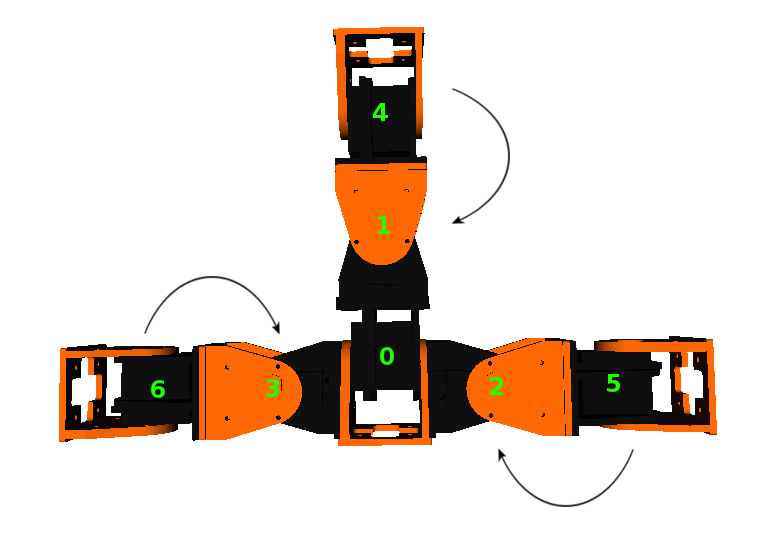
\includegraphics[width=\textwidth]{images/Hormone_protocol_tripod_step1.png}
                \caption{Step 1}
                \label{fig:tripod_step1}
        \end{subfigure}
        ~
        \begin{subfigure}[r]{0.45\textwidth}
                \centering
                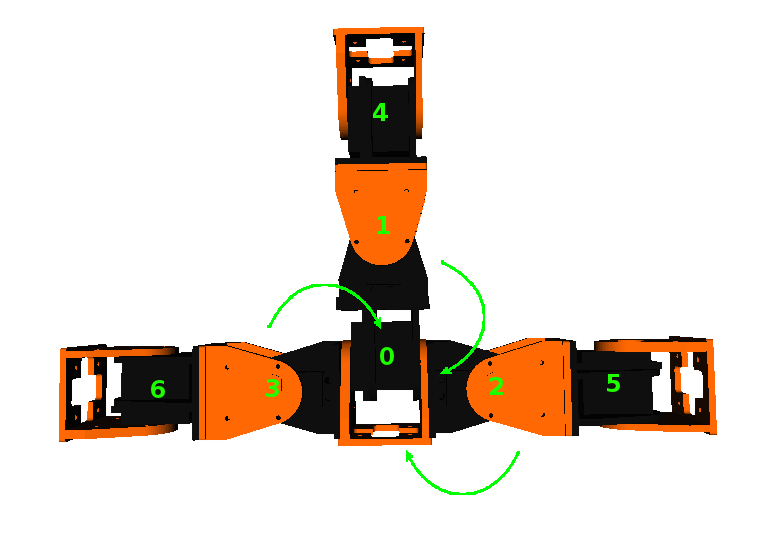
\includegraphics[width=\textwidth]{images/Hormone_protocol_tripod_step2.png}
                \caption{Step 2}
                \label{fig:tripod_step2}
        \end{subfigure}
        \caption{``Leg'' hormone flow on the \emph{MultiDof-7-Tripod} configuration}\label{fig:global_conf_discovery_tripod}
\end{figure}

Figure \ref{fig:global_conf_discovery_quad} shows the ``leg'' hormone flow through the \emph{MultiDof-9-Quad} configuration. This flow from the ``leg'' modules to the ``head'' module is completed in two steps as well, one from the modules 4, 5, 6 and 8 to the modules 1, 2, 3 and 7, and another from the modules 1, 2, 3 and 7 to the module 0, which performs the function of ``head'' module of this configuration. As it will receive 4 ``leg'' hormones in all its 4 active connectors, it will discover the module configuration to be the \emph{MultiDof-9-Quad} configuration.\\
\begin{figure}[h]
		\centering
        \begin{subfigure}[l]{0.45\textwidth}
                \centering
                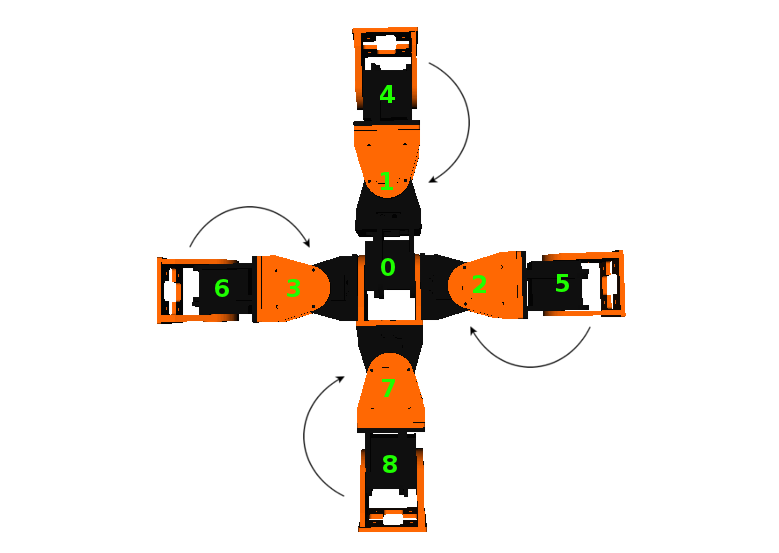
\includegraphics[width=\textwidth]{images/Hormone_protocol_quad_step1.png}
                \caption{Step 1}
                \label{fig:quad_step1}
        \end{subfigure}
        ~
        \begin{subfigure}[r]{0.45\textwidth}
                \centering
                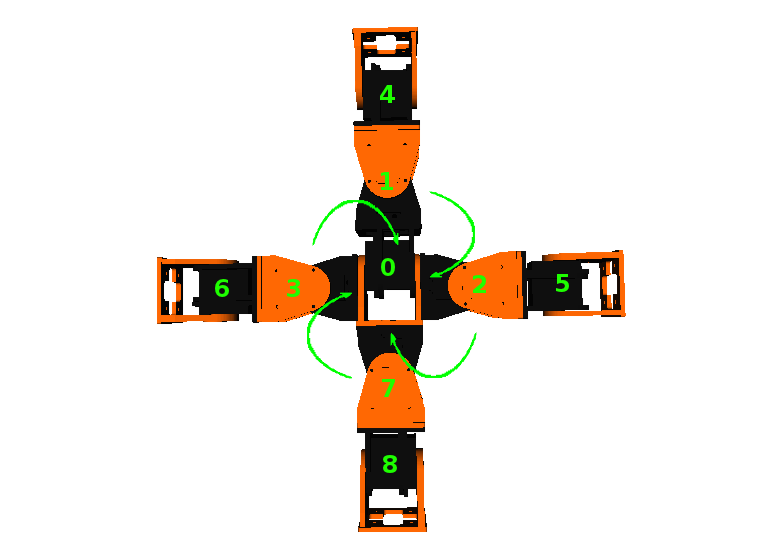
\includegraphics[width=\textwidth]{images/Hormone_protocol_quad_step2.png}
                \caption{Step 2}
                \label{fig:quad_step2}
        \end{subfigure}
        \caption{``Leg'' hormone flow on the \emph{MultiDof-9-Quad} configuration}\label{fig:global_conf_discovery_quad}
\end{figure}

The hormone flow through the \emph{MultiDof-11-2} configuration, shown in figure \ref{fig:global_conf_discovery_11_2}, is completed in one step more that the previous configurations, a total of three steps. In the first step, the modules 10, 9, 8 and 7 will send hormones to the modules 2, 3, 5 and 6. Those modules will relay the hormones to the ``shoulder'' modules, 0 and 4, and they will finally arrive to the module 1 from them, so that module 1 will become the ``head'' module of the configuration. Notice how ``head'' is a function that does not depend on the particular module, but in the configuration, and can be performed by any module when needed, as the controller is identical for all the modules. In this case, module 0 acts as ``head'' module for the \emph{MultiDof-7-Tripod} and \emph{MultiDof-9-Quad}, whereas the ``head'' of the \emph{MultiDof-11-2} configuration is the module 1.\\
\begin{figure}[h]
		\centering
        \begin{subfigure}[b]{0.4\textwidth}
                \centering
                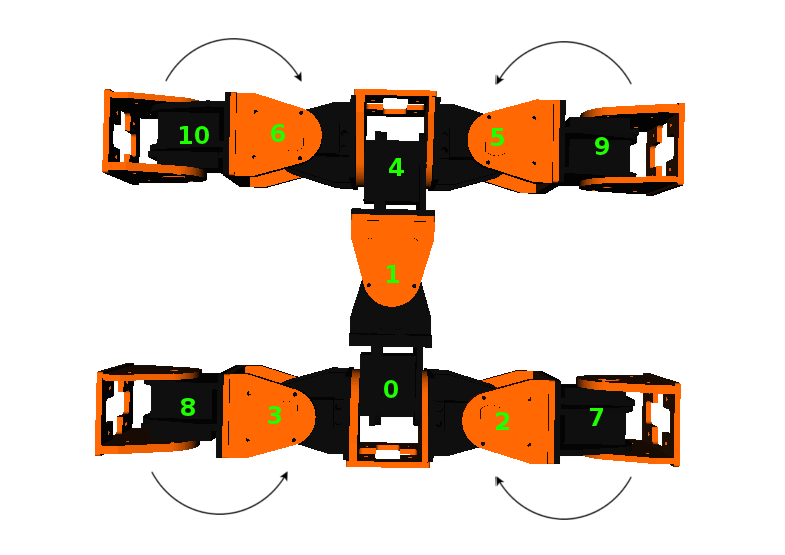
\includegraphics[width=\textwidth]{images/Hormone_protocol_11_2_step1.png}
                \caption{Step 1}
                \label{fig:11_2_step1}
        \end{subfigure}
        ~
        \begin{subfigure}[b]{0.4\textwidth}
                \centering
                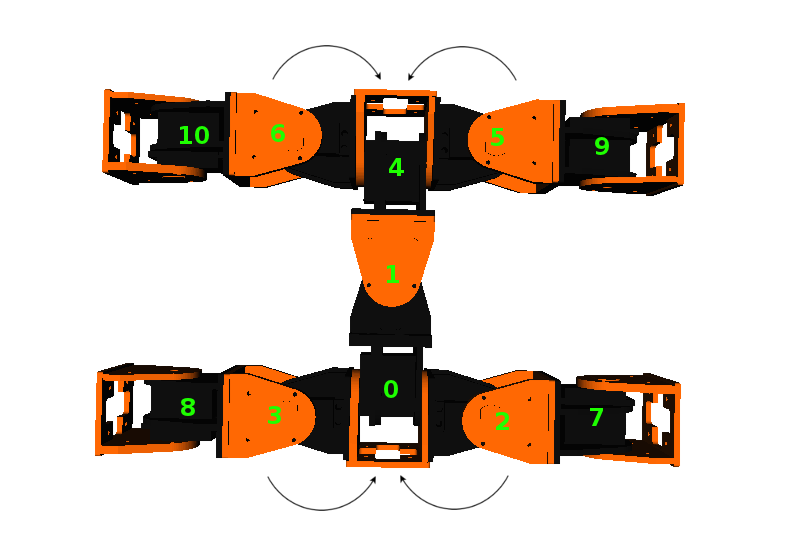
\includegraphics[width=\textwidth]{images/Hormone_protocol_11_2_step2.png}
                \caption{Step 2}
                \label{fig:11_2_step2}
        \end{subfigure}
        ~
        \begin{subfigure}[b]{0.4\textwidth}
                \centering
                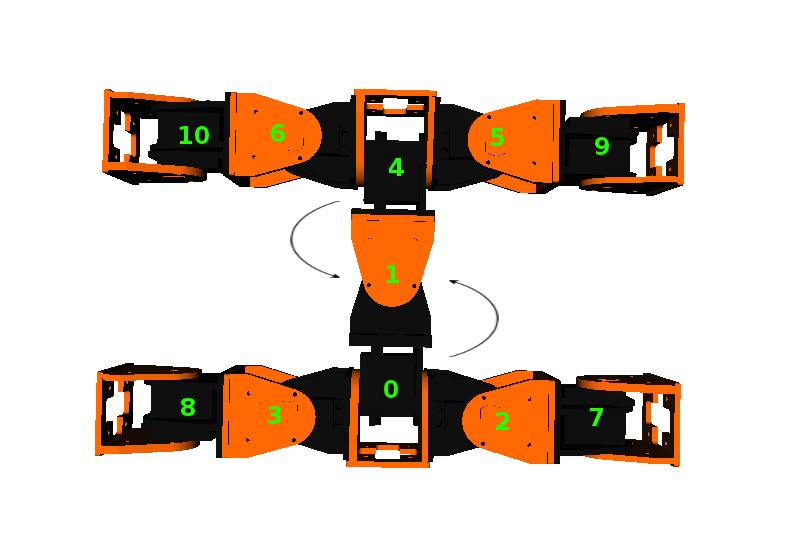
\includegraphics[width=\textwidth]{images/Hormone_protocol_11_2_step3.png}
                \caption{Step 3}
                \label{fig:11_2_step3}
        \end{subfigure}
        \caption{``Leg'' hormone flow on the \emph{MultiDof-11-2} configuration}\label{fig:global_conf_discovery_11_2}
\end{figure}


\subsubsection{Global configuration communication and leg discrimination}
\label{hormone_algorithm_head}

Once the ``head'' module has figured out which of the three possible configuration it belongs to, it will start the global configuration communication and leg discrimination algorithm.\\

As at this point only the ``head'' module knows what is the global configuration of the modular robot, so it has to communicate this information to the rest of the modules. For that purpose, it will start to generate ``head'' hormones that contain information about the current global configuration, and that will be propagated through all the modules until they arrive to the ``leg'' modules.\\

As all the ``leg'' modules have the same ID based on their connection with the neighboring modules, they also need some extra information in order to discriminate what is the position they occupy in the robot configuration. This information corresponds to an integer value from 0 to 3 that represents the connector of the ``shoulder'' module (i.e. the module that connects the limb with the body) that sent the hormone, which for the \emph{MultiDof-7-Tripod} and \emph{MultiDof-9-Quad} configurations correspond to the ``head'' module, but in the \emph{MultiDof-11-2} configuration this function is performed by the modules placed at the end of the spine (0 and 4).\\

Other important aspect to notice is that the ``leg'' modules are continuously generating hormones each step, i.e. they do not wait until the ``leg'' hormone arrives to the ``head'' module , even though not all the hormones circulating in a given step are represented on the figures, to make them clearer. This way the robot can adapt faster to changes in its global configuration, as the ``head'' module is receiving continuously information about the limbs.\\

The flow of ``head'' hormones can be observed in figures \ref{fig:global_conf_discovery_tripod_head} \ref{fig:global_conf_discovery_quad_head} and \ref{fig:global_conf_discovery_11_2_head}. Figure \ref{fig:global_conf_discovery_tripod_head} shows this flow for the \emph{MultiDof-7-Tripod} configuration. In this configuration, the ``head'' module, module 0, will generate 3 ``head'' hormones, each one of the will have in its \textbf{data} field both the code of the configuration ( `1' for \emph{MultiDof-7-Tripod}) as well as another value telling the leg which receives this hormone who has the ``head'' connector that sent the hormone.\\
% Figure for head hormones, MultiDof-7-Tripod
\begin{figure}[h]
		\centering
        \begin{subfigure}[l]{0.45\textwidth}
                \centering
                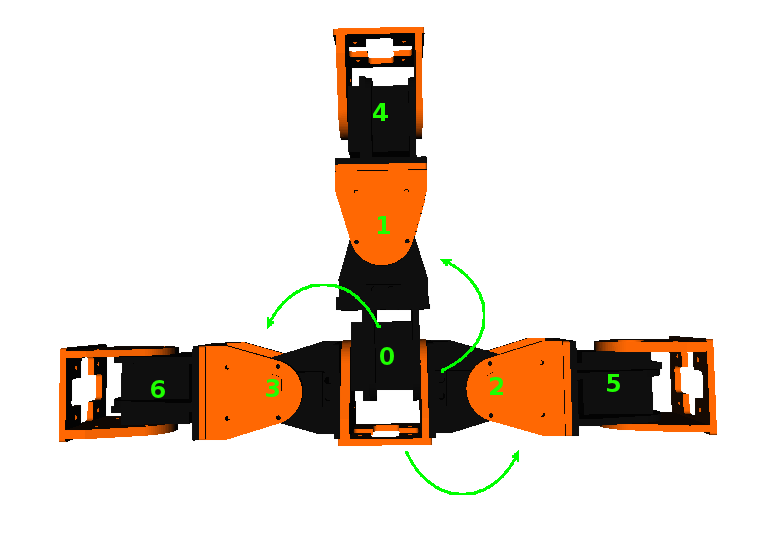
\includegraphics[width=\textwidth]{images/Hormone_protocol_tripod_head_step1.png}
                \caption{Step 1}
                \label{fig:tripod_step1_head}
        \end{subfigure}
        ~
        \begin{subfigure}[r]{0.45\textwidth}
                \centering
                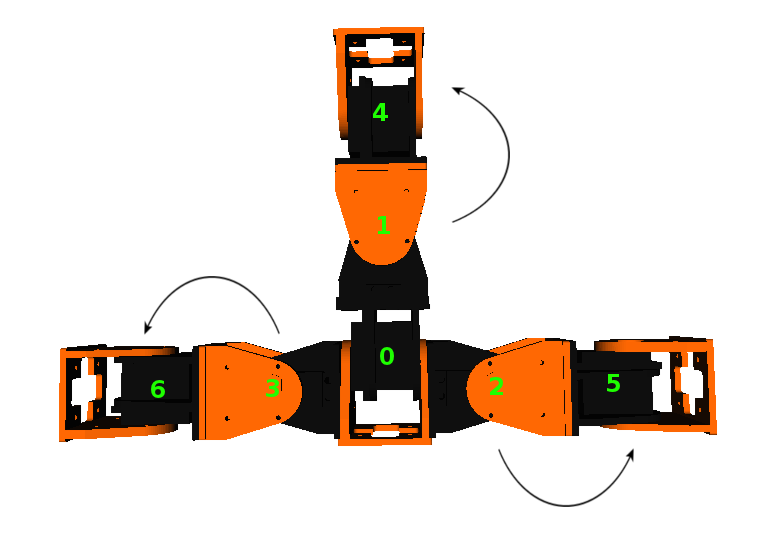
\includegraphics[width=\textwidth]{images/Hormone_protocol_tripod_head_step2.png}
                \caption{Step 2}
                \label{fig:tripod_step2_head}
        \end{subfigure}
        \caption{``Head'' hormone flow on the \emph{MultiDof-7-Tripod} configuration}\label{fig:global_conf_discovery_tripod_head}
\end{figure}

The procedure for the \emph{MultiDof-9-Quad} configuration, shown in figure \ref{fig:global_conf_discovery_quad_head}, is identical. The ``head'' module, also module 0, will generate in this case 4 ``head'' hormones, with the code of the configuration ( `2' for \emph{MultiDof-9-Quad}) and the connector that sent each hormone.\\
% Figure for head hormones, MultiDof-9-Quad
\begin{figure}[h]
		\centering
        \begin{subfigure}[l]{0.45\textwidth}
                \centering
                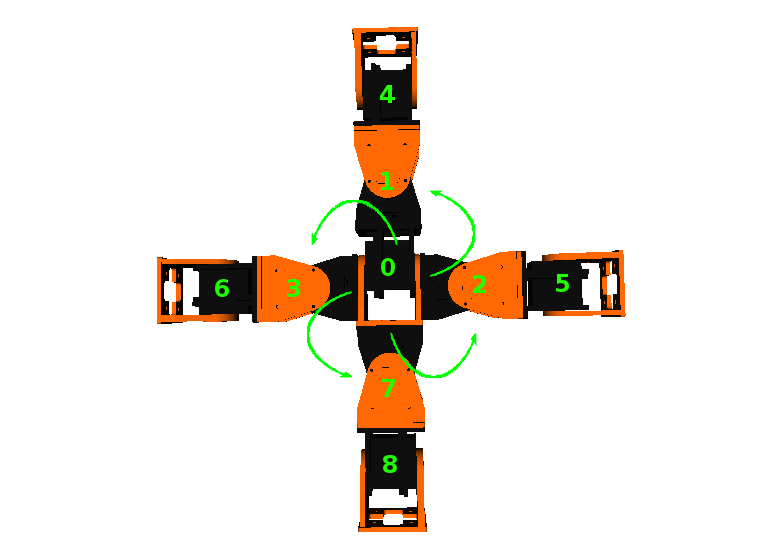
\includegraphics[width=\textwidth]{images/Hormone_protocol_quad_head_step1.png}
                \caption{Step 1}
                \label{fig:quad_step1_head}
        \end{subfigure}
        ~
        \begin{subfigure}[r]{0.45\textwidth}
                \centering
                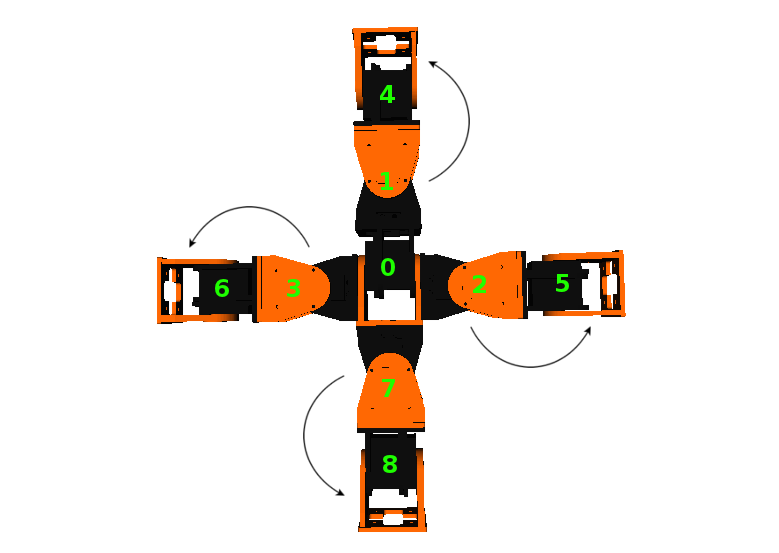
\includegraphics[width=\textwidth]{images/Hormone_protocol_quad_head_step2.png}
                \caption{Step 2}
                \label{fig:quad_step2_head}
        \end{subfigure}
        \caption{``Head'' hormone flow on the \emph{MultiDof-9-Quad} configuration}\label{fig:global_conf_discovery_quad_head}
\end{figure}

For the \emph{MultiDof-11-2} configuration, shown in figure \ref{fig:global_conf_discovery_11_2_head}, the procedure changes slightly. In this case the modules connected to the limbs are module 0 and 4, so the ``head'' module will generate ``head'' hormones with just the information about the configuration (`0' for encoding the \emph{MultiDof-11-2} configuration) on the first step. In the next step, shown in figure \ref{fig:11_2_step2_head}, and before sending the hormone to the next modules, the modules 0 and 4 will add the extra info to distinguish between the different ``leg'' modules to the hormone.\\
% Figure for head hormones, MultiDof-11-2
\begin{figure}[h]
		\centering
        \begin{subfigure}[b]{0.4\textwidth}
                \centering
                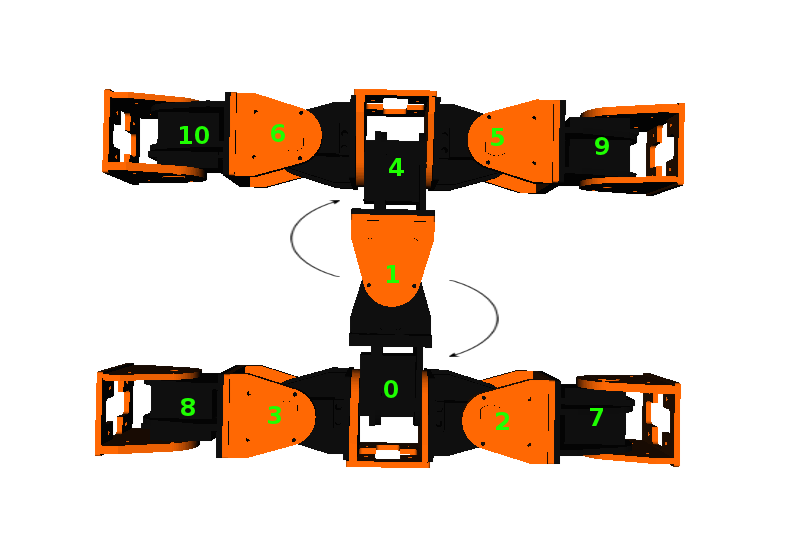
\includegraphics[width=\textwidth]{images/Hormone_protocol_11_2_head_step1.png}
                \caption{Step 1}
                \label{fig:11_2_step1_head}
        \end{subfigure}
        ~
        \begin{subfigure}[b]{0.4\textwidth}
                \centering
                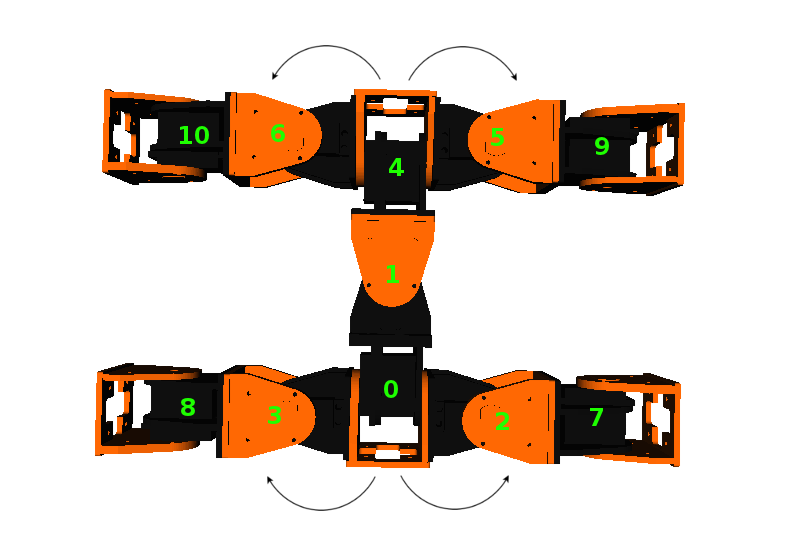
\includegraphics[width=\textwidth]{images/Hormone_protocol_11_2_head_step2.png}
                \caption{Step 2}
                \label{fig:11_2_step2_head}
        \end{subfigure}
        ~
        \begin{subfigure}[b]{0.4\textwidth}
                \centering
                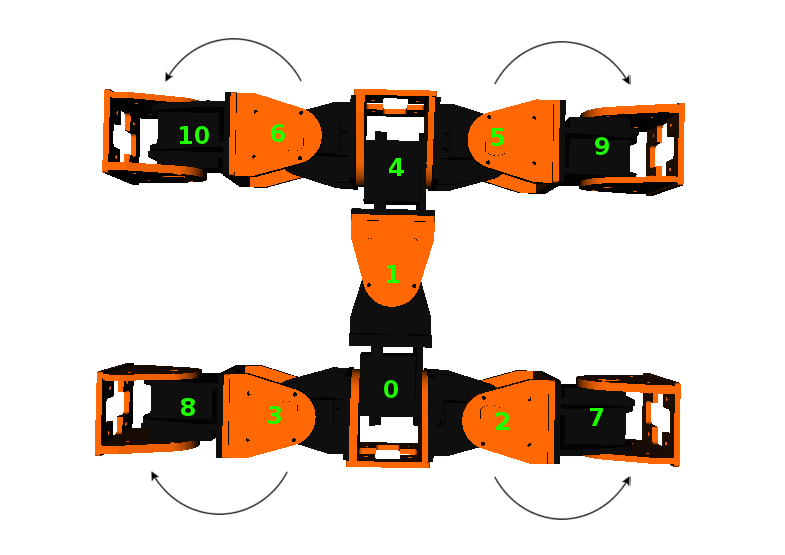
\includegraphics[width=\textwidth]{images/Hormone_protocol_11_2_head_step3.png}
                \caption{Step 3}
                \label{fig:11_2_step3_head}
        \end{subfigure}
        \caption{``Head'' hormone flow on the \emph{MultiDof-11-2} configuration}\label{fig:global_conf_discovery_11_2_head}
\end{figure}

As with the generation of ``leg'' hormones, the generation of ``head'' does not wait until the ``head'' arrives to the ``leg'' modules, but is continuously generated each time the ``leg'' hormones arrive to the ``head'' module, allowing a faster recognition of the possible changes in the global configuration.\\